\documentclass[aspectratio=169]{beamer}
\usepackage[utf8]{inputenc}

\usepackage{utopia} %font utopia imported

\usetheme{Madrid}
\usecolortheme{default}

%------------------------------------------------------------
%This block of code defines the information to appear in the
%Title page
\title[Minesweeper Solver] %optional
{Minesweeper Solver}

\subtitle{Project proposal}

\author[Team 4] % (optional)
{Chunxu Guo \and Jiahao Huang \and Qianyu Liu\\ \and Chenyang Zhang \and Tianyi Zhang}

\institute[ShanghaiTech] % (optional)
{
  ShanghaiTech University
}

\date[Dec. 14] % (optional)
{CS181: Artificial Intelligence I, Fall 2020}

\logo{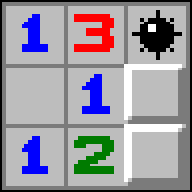
\includegraphics[height=1.0cm]{figs/icon.png}}

%End of title page configuration block
%------------------------------------------------------------



%------------------------------------------------------------
%The next block of commands puts the table of contents at the 
%beginning of each section and highlights the current section:

\AtBeginSection[]
{
  \begin{frame}
    \frametitle{Table of Contents}
    \tableofcontents[currentsection]
  \end{frame}
}
%------------------------------------------------------------


\begin{document}

%The next statement creates the title page.
\frame{\titlepage}


%---------------------------------------------------------
%This block of code is for the table of contents after
%the title page
\begin{frame}
\frametitle{Table of Contents}
\tableofcontents
\end{frame}

%---------------------------------------------------------

\section{Topic and Motivation}
% Tianyi Zhang





%---------------------------------------------------------

\section{Logic Inference}
% Qianyu Liu





%---------------------------------------------------------

\section{SAT Solver}
% Chunxu Guo





%---------------------------------------------------------

\section{CSP Probability Model}
% Jiahao Huang





%---------------------------------------------------------

\section{POMDP View}
% Chenyang Zhang

\begin{frame}
	\frametitle{POMDP Model}
	POMDP: Partially Observable Markov Decision Process
	\begin{itemize}
	    \item Generalization of a Markov decision process (MDP)
	    \item Agent cannot directly observe the underlying state
	    \item Maintain a probability distribution over the set of possible states
	\end{itemize}
\end{frame}

\begin{frame}
	\frametitle{Minesweeper POMDP Model}
	Minesweeper game can be modeled as a POMDP $<S, S_e, A, T, R, O, \Omega, b_0>$ where:

	\begin{itemize}
		\item set of states $S$: init state, normal states, failure state
		\item terminal state $S_e$: success state, failure state
		\item actions in $A$: try hidden cell $c$
		\item transition function $T$
		\item reward $R(s, a, s')$
		\item observations in $O$
		\item observation function $\Omega$: updates the knowledge matrix according to the last action
		\item $b_0$: initial probability distribution over states
	\end{itemize}
\end{frame}

\begin{frame}
	\frametitle{POMDP Challenges}
	Belief space is huge: 
	\begin{itemize}
		\item $2^{W \times H}$ states!
		\item Solving POMDPs exactly is computationally intractable
		\item MOMDP: Mixed Observability Markov Decision Process
		\begin{itemize}
			\item we can derive a compact lower-dimensional representation of the belief space
		\end{itemize}
		\item Monte-Carlo Tree Search
	\end{itemize}
\end{frame}


%---------------------------------------------------------

\section{CNN Solver}
% Tianyi Zhang





%---------------------------------------------------------

\section{\LaTeX ~ example section}

%---------------------------------------------------------
%Changing visivility of the text
\begin{frame}
\frametitle{Sample frame title}
This is a text in second frame. For the sake of showing an example.

\begin{itemize}
    \item Text 1
    \item Text 2
    \item Text 3
    \item Text 4
\end{itemize}
\end{frame}

%---------------------------------------------------------

%Example of the \pause command
\begin{frame}
In this slide \pause

the text will be partially visible \pause

And finally everything will be there
\end{frame}

%---------------------------------------------------------

%Highlighting text
\begin{frame}
\frametitle{Sample frame title}

In this slide, some important text will be
\alert{highlighted} because it's important.
Please, don't abuse it.

\begin{block}{Remark}
Sample text
\end{block}

\begin{alertblock}{Important theorem}
Sample text in red box
\end{alertblock}

\begin{examples}
Sample text in green box. The title of the block is ``Examples".
\end{examples}
\end{frame}
%---------------------------------------------------------


%---------------------------------------------------------
%Two columns
\begin{frame}
\frametitle{Two-column slide}

\begin{columns}

\column{0.5\textwidth}
This is a text in first column.
$$E=mc^2$$
\begin{itemize}
\item First item
\item Second item
\end{itemize}

\column{0.5\textwidth}
This text will be in the second column
and on a second tought this is a nice looking
layout in some cases.
\end{columns}
\end{frame}
%---------------------------------------------------------


\end{document}